\documentclass[11pt,a4paper]{article}
\usepackage[spanish,activeacute]{babel}
\decimalpoint
\usepackage[utf8]{inputenc}
\usepackage{listingsutf8}
\usepackage{amsmath}
\usepackage{amsfonts}
\usepackage{amssymb}
\usepackage{graphicx}
\usepackage{color}
\usepackage{listings}
\usepackage{amsthm}
\usepackage{caption}
\usepackage{subcaption}
\usepackage{dsfont}
\usepackage{comment}
\usepackage{enumerate}
\usepackage{mathtools,xparse}
\usepackage{ mathrsfs }
\usepackage{float}
\usepackage{listings}
\usepackage{xcolor}
\usepackage[ruled]{algorithm2e}

%% CODIGO PYTHON
\definecolor{codegreen}{rgb}{0,0.6,0}
\definecolor{codegray}{rgb}{0.5,0.5,0.5}
\definecolor{codepurple}{rgb}{0.58,0,0.82}
\definecolor{backcolour}{rgb}{0.93,0.93,0.93}

\lstdefinestyle{mystyle}{
    backgroundcolor=\color{backcolour},   
    commentstyle=\color{codegreen},
    keywordstyle=\color{magenta},
    numberstyle=\tiny\color{codegray},
    stringstyle=\color{codepurple},
    basicstyle=\ttfamily\footnotesize,
    breakatwhitespace=false,         
    breaklines=true,                 
    captionpos=b,                    
    keepspaces=true,                 
    numbers=left,                    
    numbersep=5pt,                  
    showspaces=false,                
    showstringspaces=false,
    showtabs=false,                  
    tabsize=2
}

\lstset{style=mystyle, inputencoding=utf8, extendedchars=true, literate={á}{{\'a}}1 {ó}{{\'o}}1 {é}{{\'e}}1 {ú}{{\'u}}1 {í}{{\'i}}1 {ñ}{{\~n}}1,}
%CODIGO PYTHON
\usepackage[left=2.3cm, right=2.1cm, top=2.35cm, bottom=2.35cm]{geometry}
%\renewcommand{\rmdefault}{mathpazo}
%\usepackage{mathpazo}

\usepackage[]{hyperref}
\hypersetup{
    pdftitle={Práctica 1 - MH},
    pdfauthor={Mario Muñoz Mesa},
    pdfsubject={ },
    pdfkeywords={keyword1, keyword2},
    bookmarksnumbered=true,     
    bookmarksopen=true,         
    bookmarksopenlevel=1,       
    colorlinks=true,   
    linkcolor=black,         
    pdfstartview=Fit,           
    pdfpagemode=UseOutlines,
    pdfpagelayout=TwoPageRight
}


\DeclarePairedDelimiter{\norm}{\lVert}{\rVert}
\NewDocumentCommand{\normL}{ s O{} m }{%
  \IfBooleanTF{#1}{\norm*{#3}}{\norm[#2]{#3}}_{L_2(\Omega)}%
}

\DeclareMathOperator*{\argmax}{arg\,max}
\DeclareMathOperator*{\argmin}{arg\,min}

\newtheorem{theorem}{Teorema}

\theoremstyle{definition}
\newtheorem{definition}{Definición}[section]


\newtheorem{proposition}{Proposición}[section]


\newtheorem{corolary}{Corolario}[section]


\newtheorem{lema}{Lema}[section]

	\newcommand{\R}{\mathbb{R}}
	\newcommand{\N}{\mathbb{N}}
	\newcommand{\C}{\mathbb{C}}


\title{
\normalfont \normalsize 
\textsc{\small METAHEURÍSTICAS} \\ [10pt]
	
	
\huge{\textbf{Práctica 1 - APC}}\\

\textsc{\small Grupo 1} \\ [10pt]

	}

\author{Mario Muñoz Mesa\\ mario43514@correo.ugr.es}
\date{\today}


\begin{document}
	\maketitle
	\newpage
	\renewcommand*\contentsname{Índice}	
	\tableofcontents
	
	\newpage
	
	\section{Descripción del problema.}
	Nos ocupamos del problema del Aprendizaje de Pesos en Características (APC). Plantea, en el contexto de un problema de clasificación, elegir o ajustar un vector de pesos $\textbf{w}=(w_1,\ldots, w_d)\in [0,1]^d$ asociado a las características en base a un criterio de mejora del clasificador. Hemos denotado con $d$ al número de características.\\
	
	En nuestro caso trabajaremos con clasificador tipo 1-NN, y el criterio será maximizar:
	$$F(\textbf{w}):=\alpha\cdot \text{tasa\_clas}(\textbf{w})+(1-\alpha ) \cdot \text{tasa\_red}(\textbf{w})$$
	donde
	$$\text{tasa-clas}:=100\frac{\text{nº instancias bien clasificadas en training}}{\text{nº instancias en training}}, \quad \quad \text{tasa-red}:=100\frac{\text{nº valores } w_i <0.2}{\text{nº características}}$$
	y $alpha=0.5$ que pondera la importancia entre el acierto y la reducción de características para el nuevo mejor clasificador que se pretende encontrar.\\
	
	De lo que nos ocupamos por tanto es de obtener $\argmax_{\textbf{w}\in [0,1]^d} F(\textbf{w})$ para un clasificador 1-NN que utilizará la distancia ponderada
	$$d_{\textbf{w}}(u,v)=\sqrt{\sum_{i=1}^d w_i(u_i-v_i)^2}, \quad u,v\in \R^d$$
	para clasificar. Queremos que aumente el acierto y reduzca el número de características, cualquier característica con peso menor estricto a 0.2 se descarta.
	
	
	\newpage
	\section{Descripción de la aplicación de los algoritmos empleados.}
	\subsection{Asociados al preprocesado y representación.}
	Partimos de un conjunto de entrenamiento $T$ formado por instancias de una muestra. Cada instancia se ha representado mediante una estructura de datos \texttt{SampleElement} que recoge las valores de las características en un vector \texttt{vector<double>} y la clase como una cadena de caracteres.
	
	De esta forma, cada dataset se lee mediante la función \texttt{read\_arff} y lo almacenamos como un vector de elementos muestrales \texttt{vector<SampleElement>}. 
	
	Para la normalización utilizamos min-max normalization, se ha implementado en \texttt{normalization}.
	
	Las particiones para la validación cruzada $k-fold$ se realizan respetando la proporción de clases en cada partición, para ello cada elemento de una clase se va asignando a una partición de forma cíclica.
	
	La solución será un vector de pesos con valores entre 0 y 1, cada componente indica el peso de una característica, se representa como un \texttt{vector<double>}
	\subsection{Funciones generales.}
	Nuestro clasificador utiliza la distancia euclídea, para manejarla se han implementado dos funciones: \texttt{euclidean\_distance2} y \texttt{euclidean\_distance2\_w}.
	
	
	\begin{algorithm}
		\caption{euclidean\_distance2}
		\KwIn{vector de reales $a$, vector de reales $b$}
		\KwOut{la distancia euclídea al cuadrado entre $a$ y $b$}
		\Begin{
			dist $\leftarrow$ 0
			
			\For { $i=0$ to $a.size()-1$ }{
				dist $\leftarrow$ dist + $(a[i]-b[i])^2$
			}
			\Return dist
		}
	\end{algorithm}
	
	\begin{algorithm}
		\caption{euclidean\_distance2\_w}
		\KwIn{vector de reales $a$, vector de reales $b$, vector de pesos $weights$}
		\KwOut{la distancia euclídea ponderada y al cuadrado entre $a$ y $b$}
		\Begin{
			dist $\leftarrow$ 0
			
			\For { $i=0$ \textbf{to} $a.size() -1$ }{
			\tcp{se descartan las características con peso < 2}	
				\If{$weights[i] \geq 0.2$}{ 
				dist $\leftarrow$ dist + $(a[i]-b[i])^2$
				}
			}
			\Return dist
		}
	\end{algorithm}
	La función \texttt{euclidean\_distance2}  se utiliza exclusivamente para el cálculo de amigo y enemigo más cercano en el algoritmo Relief. Con \texttt{euclidean\_distance2\_w} calculamos la distancia ponderada descartando pesos menores a 0.2, se utiliza en 1-NN y Búsq. Local.
	
	En ambos casos calculamos la distancia euclídea al cuadrado por motivos de eficiencia y porque lo que nos interesa es comparar distancias, y como la raíz cuadrada es una función creciente, si $a>b$ $\Rightarrow $ $\sqrt{a}>\sqrt{b}$, no hay inconveniente en trabajar con la distancia al cuadrado.
	
	El algoritmo 1-NN, haciendo uso de distancia ponderada, se ha implementado en \texttt{one\_NN}.
	
	\begin{algorithm}
		\caption{one\_NN}
		\KwIn{elemento muestral $sam\_el$ a clasificar, conjunto de elementos muestrales sobre el que buscar el más cercano $sam\_elements$, vector de pesos $weights$}
		\KwOut{la clase o etiqueta del elemento más cercano, $min\_l$}
		\Begin{
			$min\_dist \leftarrow \infty$
			
			\For { $e$ \textbf{in} $sam\_elements$ }{
				$d\leftarrow$ euclidean\_distance2\_w(e.features, sam\_el.features, weights)
				
				\If{$d < min\_dist$}{
					$min\_l$ $\leftarrow$ e.label\\
					$min\_dist \leftarrow d$
				}
			}
			\Return min\_l
		}
	\end{algorithm}
	
	La versión con leave-one-out, que se utiliza en Búsq. Local, simplemente consiste en dejar un elemento fuera.
	
	\begin{algorithm}
		\caption{one\_NN\_lo}
		\KwIn{elemento muestral $sam\_el$ a clasificar, conjunto de elementos muestrales sobre el que buscar el más cercano $sam\_elements$, vector de pesos $weights$, posición de elemento a dejar fuera $leave\_out$}
		\KwOut{la clase o etiqueta del elemento más cercano, $min\_l$}
		\Begin{
			$min\_dist \leftarrow \infty$
			
			\For { $i=0$ \textbf{to} $sam\_elements.size()-1$ }{
			\If{$i\neq leave\_out$}{
				$d\leftarrow$ euclidean\_distance2\_w(sam\_elements[i].features, sam\_el.features, weights)
				
				\If{$d < min\_dist$}{
					$min\_l$ $\leftarrow$ sam\_elements[i].label\\
					$min\_dist \leftarrow d$
				}
			}
			}
			\Return min\_l
		}
	\end{algorithm}
	
	\subsection{Función objetivo.}
	Para el cálculo de las tasas se han implementado las funciones \texttt{class\_rate} y \texttt{red\_rate} que simplemente implementan la propia de definición de tasa-class y tasa-red.\\
	
	\begin{algorithm}[H]
		\caption{class\_rate}
		\KwIn{vector con clases o etiquetas de elementos clasificados $class\_labels$, elementos de test $test$}
		\KwOut{el porcentaje de acierto}
		\Begin{
			$n\leftarrow 0$\\
  			$class\_labels\_s \leftarrow class\_labels.size()$
  			
			\For { $i=0$ \textbf{to} $class\_labels\_s-1$ }{
			\If{$class\_labels\_s[i] == test[i].label$}{
				$n\leftarrow n+1$
			}

			}
			
			\Return $100\frac{n}{class\_labels\_n}$
		}
	\end{algorithm}~\\
	
	\begin{algorithm}[H]
		\caption{red\_rate}
		\KwIn{vector de pesos $weights$}
		\KwOut{el porcentaje de reducción}
		\Begin{
			$feats\_reduced \leftarrow 0$
			
			\For { $w$ \textbf{in} $weights$ }{
			\If{$w < 0.2$}{
				$feats\_reduced \leftarrow feats\_reduced+1$
			}

			}
			
			\Return $100\frac{feats\_reduced}{initial\_number\_of\_features}$
		}
	\end{algorithm} ~\\
	
	La función objetivo, teniendo en cuenta que trabajamos con $\alpha=0.5$, nos quedaría:\\
	
	\begin{algorithm}[H]
		\caption{obj\_function}
		\KwIn{tasa de clasificación $class\_rate$, tasa de reducción $red\_rate$}
		\KwOut{el valor de la función objetivo o fitness}
		\Begin{
			
			\Return $\alpha \cdot class\_rate + (1-\alpha) \cdot red\_rate$
		}
	\end{algorithm}
	
	\section{Descripción de los algoritmos.}
	\subsection{RELIEF (Greedy).}
	Este algoritmo será el de comparación. El objetivo es generar un vector de pesos a partir de las distancias de cada ejemplo o elemento al amigo (misma clase) y enemigo (clase distinta) más cercano.
	
	La idea subyacente es, para cada característica, premiar en peso la lejanía de un ejemplo a su enemigo más cercano (separa bien), y penalizar la lejanía de un ejemplo a su amigo más cercano.
	
	Se comienza con vector de pesos 0. Se recorren los elementos de entrenamiento, identificando enemigo y amigo más cercano, y se actualizan las componentes de los pesos sumando la distancia del enemigo más cercano y restando la del amigo más cercano en cada característica. Luego se restringen los pesos a $[0,1]$ truncando los valores negativos a 0 y normalizando el resto dividiendo por el máximo peso en el vector de pesos.
	
	Para la implementación se ha creado previamente la función \texttt{closest\_friend\_enemy} que busca el amigo y enemigo más cercanos a un elemento.~\\
	
	\begin{algorithm}[H]
		\caption{closest\_friend\_enemy}
		\KwIn{posición del elemento $pos$, conjunto de entrenamiento $training$, elemento que será el amigo más cercano $friend\_e$, elemento que será el enemigo más cercano $enemy\_e$}
		\Begin{
			$min\_friend\_d \leftarrow \infty$\\
			$min\_enemy\_d \leftarrow \infty$
			
			\For{$i \in \{0,\ldots ,pos-1, pos+1,\ldots , training.size()-1\}$}{
				$distance\leftarrow  euclidean\_distance2(training[i].features, training[pos].features) $
				
			\If{elemento i y elemento pos son amigos}{
				\If{$distance < min\_friend\_d$}{
					$min\_friend\_d \leftarrow distance$\\
					$min\_friend\_p \leftarrow i$
				}
			}
			\Else{
				\If{$distance < min\_enemy\_d$}{
					$min\_enemy\_d \leftarrow distance$\\
					$min\_enemy\_p \leftarrow i$
				}
			}
		}
		$friend\_e \leftarrow training[min\_friend\_p]$\\
		$enemy\_e \leftarrow training[min\_enemy\_p]$\\
		}
	\end{algorithm}~\\
	
	
	El agoritmo RELIEF:~\\
	
	\begin{algorithm}[H]
		\caption{relief}
		\KwIn{conjunto de elementos muestrales $training$}
		\KwOut{vector de pesos $weights$}
		\Begin{
			$weights \leftarrow (0,\ldots ,0)$\\
			\tcp{se va buscando enemigo y amigo más cercano para cada elemento}
			\For{$i=0$ \textbf{to} $training.size()-1$}{
				$closest\_friend\_enemy(i, training, friend, enemy) $\\
			\tcp{se actualizan los pesos}
			\For{$j=0$ \textbf{to} $num\_feats-1$}{
				\If{$distance < min\_friend\_d$}{
					$weights[j]\leftarrow weights[j]+|training[i].features[j]-enemy.features[j]| - |training[i].features[j]-friend.features[j]|$
				}
			}

			}
			$max\_weight \leftarrow \max_{i\in \{0,\ldots , num\_feats -1\} } weights[i]$\\
			\tcp{se restringe a [0,1]}
			\For{$j=0$ \textbf{to} $num\_feats$}{
				\If{$weights[j] < 0$}{
					$weights[j] \leftarrow 0$				
				}
				\Else{
					$weights[j]\leftarrow \frac{weights[j]}{max\_weight}$				
				}			
			}
			\Return weights

		}
	\end{algorithm}
	\subsection{Búsqueda Local.}
	Para la Búsqueda Local se emplea la estrategia del primer mejor. \iffalse La idea es escoger la primera solución vecina (vector de pesos) que mejore la función objetivo actual.\fi La idea es generar soluciones (vectores de pesos) vecinas hasta encontrar la primera mejor que la actual, en ese caso se sustituye la actual por la encontrada. Este proceso es iterativo.
	
	Para ello se parte de una solución (vector de pesos) inicial; se toman valores de una distribución uniforme $\mathcal{U}(0,1)$.
	
	Para generar las soluciones vecinas, se va eligiendo una componente aleatoria sin repetición. Las soluciones vecinas se generan mutando el vector de pesos actual al sumar un elemento de una distribución normal de media 0 y desviación típica 0.3 (pesos fueras del rango [0,1] se truncan). Si se mejora la función objetivo con el nuevo vector de pesos, éste pasará a ser el actual. Además, en ese caso, o en el caso de haber recorrido todas las componentes, se establece un nuevo orden aleatorio de las componentes a recorrer.
	
	Este proceso se repite iterativamente hasta alcanzar 15000 evaluaciones de la función objetivo o hasta la generación de un número de vecinos igual a 20 veces el número de características.
	

	Para representar los índices de componentes del vector de pesos, que eventualmente se mezclan según lo anterior, se ha construido un vector de enteros. Este vector junto con el vector de pesos se inicializan en la función \texttt{rand\_init\_sol\_gen\_indexes}~\\
	
	\begin{algorithm}[H]
		\caption{rand\_init\_sol\_gen\_indexes}
		\KwIn{vector en el que inicializar los pesos $weights$, vector de índices $indexes$}
		\Begin{
			\For{$i=0$ \textbf{to} $number\_of\_features-1$}{
				$weights.push\_back(e\in \mathcal{U}(0,1))$\\
				$indexes.push\_back(i)$
			}

		}
	\end{algorithm}~\\
	
	También hemos construido una función que realiza la mutación en el vector de pesos:~\\
	
	\begin{algorithm}[H]
		\caption{mutation}
		\KwIn{vector de pesos $weights$, índice a mutar $i$, distribución normal $n\_dist$}
		\Begin{
		$weights[i] \leftarrow weights[i] + e\in \mathcal{N}_{n\_dist}(0,0.3)$\\
		\If{$weigths[i]>1$}{
			$weights[i]\leftarrow 1$		
		}
		\Else{
			\If{$weights[i]<0$}{
				$weights[i]\leftarrow 0$			
			}		
		}
		}
	\end{algorithm}~\\
	
	Y una función que clasifica un conjunto de elementos mediante leave one out, con distancia ponderada, y obtiene el correspondiente valor de la función objetivo para esa clasificación:~\\ 
	
	\begin{algorithm}[H]
		\caption{classifyloo\_and\_objf}
		\KwIn{elementos de entrenamiento conjunto de entrenamiento $training$, vector de pesos $weights$, vector a contener las etiquetas de clasificación $class\_labels$}
		\KwOut{el valor de la función objetivo de la clasificación, $obj$}
		\Begin{
		\For{$k=0$ \textbf{to} $training.size()-1$}{
			$class\_labels.push\_back(one\_NN\_lo(training[k], training, weights, k))$
		}
		$obj\leftarrow obj\_function(class\_rate(class\_labels, training), red\_rate(weights))$\\
		$class\_labels.clear()$
		
		\Return $obj$
		
		}
	\end{algorithm}~\\
	
	Finalmente tenemos la función que realiza la búsqueda local:~\\
	
	\begin{algorithm}[H]
		\caption{local\_search}
		\KwIn{conjunto de elementos muestrales $training$}
		\KwOut{mejor vector de pesos alcanzado $weights$}
		\Begin{
			$rand\_init\_sol\_gen\_indexes(best\_weights, comp\_indexes)$\\
			\tcp{clasificamos con los mejores pesos hasta el momento mediante leave one out, y obtenemos valor de la función objetivo}
			$best\_obj \leftarrow classifyloo\_and\_objf(training, best\_weights, class\_labels)$\\ ~\\
			
			\While{$gen\_neighbours < max\_gen\_neighbours$ \textbf{and} $obj\_eval\_count < max\_objf\_evals$}{
			\tcp{aleatorizamos componentes a mutar si se han recorrido todas o se mejoró f.obj}
			\If{$new\_best\_obj$ \textbf{or} $mod\_pos \% number\_of\_features == 0$}{
				$new\_best\_obj \leftarrow false$\\
				$shuffle(comp\_indexes)$\\
				$mod\_pos \leftarrow 0$
			}
			\tcp{Se toma componente a mutar y se muta}
			$comp\_to\_mut \leftarrow comp\_indexes[mod\_pos \% number\_of\_features]$
			
			$muted\_weights \leftarrow best\_weights$
			
			$mutation(muted\_weights, comp\_to\_mut, n\_dist)$\\
			
			$gen\_neighbours \leftarrow gen\_neighbours +1$\\
			\tcp{clasificamos con los nuevos pesos mutados mediante leave one out, y obtenemos valor de la función objetivo}
			$obj \leftarrow classifyloo\_and\_objf(training, muted\_weights, class\_labels)$\\
			\tcp{Si se ha mejorado, actualizamos mejor objetivo y weights, y vecinos generados}
			\If{$obj>best\_obj$}{
				$best\_weights \leftarrow muted\_weights$\\
				$best\_obj \leftarrow obj$\\
				$gen\_neighbours \leftarrow 0$\\
				$new\_best\_obj \leftarrow true$
			}
			
			$obj\_eval\_count\leftarrow obj\_eval\_count+1$\\
			$mod\_pos\leftarrow mod\_pos +1$
			}
					
			
			\Return $best\_weights$
		}
		
	\end{algorithm}
	
	

	\section{Procedimiento considerado en el desarrollo.}
	Para el desarrollo de la práctica no se ha utilizado ningún framework, se han implementado las funciones necesarias en C++. Todo el código se encuentra en \texttt{p1.cpp}.
	
	Para la ejecución basta indicar un argumento con el archivo a ejecutar, en este caso se utiliza la semilla por defecto 1234, que es la misma que se utilizó para los resultados de esta memoria.
	
	También se incluye un fichero \texttt{p1\_all\_datasets.sh} que ejecuta, con la semilla por defecto, \texttt{p1} sobre los 3 datasets.
	\section{Experimentos y análisis de resultados.}
	Los 3 datasets con los que se ha trabajado son:
	\begin{itemize}
		\item \textbf{Ionosphere}: Conjunto de datos de radar que fueron recogidos por un sistema \textit{Goose Bay}, Labrador. Consta de 352 instancias con 34 características y 2 clases.
		\item \textbf{Parkinsons}: Conjunto de datos orientado a distinguir entre la presencia y ausencia de la enfermedad de Parkinson. Consta de 195 ejemplos con 22 características y 2 clases.
		\item \textbf{Spectf-Heart}: Conjunto de datos de detección de enfermedades cardiacas a partir de imágenes médicas de tomografía computerizada del corazón de pacientes. Consta de 267 ejemplos con 44 características y 2 clases.
	\end{itemize}
	
	Los resultados obtenidos son:~\\
	
	\textbf{1-NN}

	\begin{tabbing}
	\resizebox{\textwidth}{!}{%
		\begin{tabular}{|c|}
			\hline \textbf{Nº}\\ \textbf{part.} 
			\\ \hline
			\textbf{P1} \\ \hline 
			\textbf{P2} \\ \hline
			\textbf{P3} \\ \hline 
			\textbf{P4} \\ \hline
			\textbf{P5} \\ \hline
			\textbf{Media} \\ \hline
		\end{tabular}
		\begin{tabular}{|c|c|c|c|}
			\hline
			\multicolumn{4}{|c|}{\textbf{Ionosphere}} \\ \hline
			\textbf{\%clas} & \textbf{\%red} & \textbf{Agr.} & \textbf{T} \\ \hline 
			87.3239	&0	&43.662	&0.373 \\ \hline
64.2857	&0	&32.1429&	0.325 \\ \hline
64.2857	&0	&32.1429&	0.325 \\ \hline
64.2857	&0	&32.1429&	0.325 \\ \hline
64.2857	&0	&32.1429&	0.381 \\ \hline
68.89334	&0	&34.44672	&0.3458 \\ \hline
		\end{tabular}
		
		\begin{tabular}{|c|c|c|c|}
			\hline
			\multicolumn{4}{|c|}{\textbf{Parkinsons}} \\ \hline
			\textbf{\%clas} & \textbf{\%red} & \textbf{Agr.} & \textbf{T} \\ \hline 
95	      &0	&47.5	   & 0.181\\ \hline
25	      &0	&12.5	   & 0.073\\ \hline
25.641	  &0	&12.8205	&  0.072\\ \hline
23.6842	  &0	&11.8421	&  0.07\\ \hline
23.6842	  &0	&11.8421	&  0.071\\ \hline
38.60188	&0	&19.30094&	0.0934\\ \hline

		\end{tabular}
		
		\begin{tabular}{|c|c|c|c|}
			\hline
			\multicolumn{4}{|c|}{\textbf{Spectf-Heart}} \\ \hline
			\textbf{\%clas} & \textbf{\%red} & \textbf{Agr.} & \textbf{T} \\ \hline 
			85.7143	&0	&42.8571	&  0.468\\ \hline
72.8571	&0	&36.4286	&  0.407\\ \hline
72.8571	&0	&36.4286	&  0.397\\ \hline
72.8571	&0	&36.4286	&  0.397\\ \hline
73.5294	&0	&36.7647	&  0.388\\ \hline
75.563	&0	&37.78152&	0.4114\\ \hline

		\end{tabular}
		}
	\end{tabbing}
	
	\textbf{Relief}
	
		\begin{tabbing}
	\resizebox{\textwidth}{!}{%
		\begin{tabular}{|c|}
			\hline \textbf{Nº}\\ \textbf{part.} 
			\\ \hline
			\textbf{P1} \\ \hline 
			\textbf{P2} \\ \hline
			\textbf{P3} \\ \hline 
			\textbf{P4} \\ \hline
			\textbf{P5} \\ \hline
			\textbf{Media} \\ \hline
		\end{tabular}
		\begin{tabular}{|c|c|c|c|}
			\hline
			\multicolumn{4}{|c|}{\textbf{Ionosphere}} \\ \hline
			\textbf{\%clas} & \textbf{\%red} & \textbf{Agr.} & \textbf{T} \\ \hline 
			88.7324	&  2.94118&	45.8368	 & 1.753\\ \hline
			84.2857	&  5.88235&	45.084	  &1.757\\ \hline
			90    	 & 2.94118	&46.4706	  &1.76\\ \hline
			88.5714	&  2.94118&	45.7563	 & 1.761\\ \hline
			87.1429	&  2.94118&	45.042	  &1.766\\ \hline
			87.74648&	3.529414& 45.63794	&1.7594\\ \hline

		\end{tabular}
		
		\begin{tabular}{|c|c|c|c|}
			\hline
			\multicolumn{4}{|c|}{\textbf{Parkinsons}} \\ \hline
			\textbf{\%clas} & \textbf{\%red} & \textbf{Agr.} & \textbf{T} \\ \hline 
			95	      &9.09091	  &52.0455	  &0.364\\ \hline
97.5	    &4.54545	  &51.0227	  &0.366\\ \hline
94.8718	  &4.54545	  &49.7086	  &0.371\\ \hline
92.1053	  &4.54545	  &48.3254	  &0.369\\ \hline
100	      &0	        &50	        &0.374\\ \hline
95.89542	&4.545452	  &50.22044	  &0.3688\\ \hline
		\end{tabular}
		
		\begin{tabular}{|c|c|c|c|}
			\hline
			\multicolumn{4}{|c|}{\textbf{Spectf-Heart}} \\ \hline
			\textbf{\%clas} & \textbf{\%red} & \textbf{Agr.} & \textbf{T} \\ \hline 
			90	      &0	&45	      &2.28\\ \hline
87.1429	  &0	&43.5714	  &2.222\\ \hline
80	      &0	&40	      &2.201\\ \hline
84.2857	  &0	&42.1429	  &2.172 \\ \hline
77.9412	  &0	&38.9706	  &2.237 \\ \hline
83.87396	&0	&41.93698	&2.2224\\ \hline

		\end{tabular}
		}
	\end{tabbing}
	
	\textbf{Búsqueda Local}
	
		\begin{tabbing}
	\resizebox{\textwidth}{!}{%
		\begin{tabular}{|c|}
			\hline \textbf{Nº}\\ \textbf{part.} 
			\\ \hline
			\textbf{P1} \\ \hline 
			\textbf{P2} \\ \hline
			\textbf{P3} \\ \hline 
			\textbf{P4} \\ \hline
			\textbf{P5} \\ \hline
			\textbf{Media} \\ \hline
		\end{tabular}
		\begin{tabular}{|c|c|c|c|}
			\hline
			\multicolumn{4}{|c|}{\textbf{Ionosphere}} \\ \hline
			\textbf{\%clas} & \textbf{\%red} & \textbf{Agr.} & \textbf{T} \\ \hline 
			78.8732	&85.2941	&82.0837	  &3311.36\\ \hline
92.8571	&85.2941	&89.0756	  &4673.61\\ \hline
95.7143	&82.3529	&89.0336	  &1986.46\\ \hline
88.5714	&88.2353	&88.4034	  &3914.9\\ \hline
90	    &85.2941	&87.6471	  &2388.89\\ \hline
89.2032&	85.2941&	87.24868	&3255.044\\ \hline

		\end{tabular}
		
		\begin{tabular}{|c|c|c|c|}
			\hline
			\multicolumn{4}{|c|}{\textbf{Parkinsons}} \\ \hline
			\textbf{\%clas} & \textbf{\%red} & \textbf{Agr.} & \textbf{T} \\ \hline 
			87.5	 &86.3636	  &86.9318&	390.064\\ \hline
82.5	 &90.9091	  &86.7045&	408.803\\ \hline
87.1795	&86.3636	  &86.7716&	339.172\\ \hline
86.8421&	50	      &68.4211&	265.049\\ \hline
97.3684&	86.3636	 & 91.866&	581.204\\ \hline
88.278&	79.99998	&84.139	&396.8584\\ \hline

		\end{tabular}
		
		\begin{tabular}{|c|c|c|c|}
			\hline
			\multicolumn{4}{|c|}{\textbf{Spectf-Heart}} \\ \hline
			\textbf{\%clas} & \textbf{\%red} & \textbf{Agr.} & \textbf{T} \\ \hline 
			85.7143	 & 88.6364	&87.1753	 & 6719.91 \\ \hline
85.7143	&  86.3636&	86.039	 & 7458.06 \\ \hline
88.5714	 & 88.6364	&88.6039	 & 5512.85 \\ \hline
85.7143	 & 77.2727	&81.4935	 & 3448.21 \\ \hline
80.8824	 & 88.6364	&84.7594	 & 3612.81 \\ \hline
85.31934&	85.9091	&85.61422	&5350.368 \\ \hline
		\end{tabular}
		}
	\end{tabbing}
	
	Y la tabla resumen:
	\begin{tabbing}
	\resizebox{\textwidth}{!}{%
		\begin{tabular}{|c|}
			\hline \textbf{Nº}\\ \textbf{part.} 
			\\ \hline
			\textbf{1-NN} \\ \hline 
			\textbf{Relief} \\ \hline
			\textbf{Búsq. Local} \\ \hline 
		\end{tabular}
		\begin{tabular}{|c|c|c|c|}
			\hline
			\multicolumn{4}{|c|}{\textbf{Ionosphere}} \\ \hline
			\textbf{\%clas} & \textbf{\%red} & \textbf{Agr.} & \textbf{T} \\ \hline 
			68.89334	&0	          &34.44672	&0.3458\\ \hline
87.74648&	3.529414	  &45.63794	&1.7594\\ \hline
89.2032	  &85.2941	    &87.24868	&3255.044\\ \hline
		\end{tabular}
		
		\begin{tabular}{|c|c|c|c|}
			\hline
			\multicolumn{4}{|c|}{\textbf{Parkinsons}} \\ \hline
			\textbf{\%clas} & \textbf{\%red} & \textbf{Agr.} & \textbf{T} \\ \hline 
			38.60188	&0	        &19.30094	&0.0934\\ \hline
95.89542&	4.545452	&50.22044	&0.3688\\ \hline
88.278	 & 79.99998	&84.139	  &396.8584\\ \hline

		\end{tabular}
		
		\begin{tabular}{|c|c|c|c|}
			\hline
			\multicolumn{4}{|c|}{\textbf{Spectf-Heart}} \\ \hline
			\textbf{\%clas} & \textbf{\%red} & \textbf{Agr.} & \textbf{T} \\ \hline 
			75.563	  &0	      &37.78152	&0.4114\\ \hline
83.87396	&0	      &41.93698	&2.2224\\ \hline
85.31934	&85.9091	&85.61422	&5350.368\\ \hline
		\end{tabular}
		}
	\end{tabbing}~\\
	


	
	En cuanto a las tasas, en primer lugar vemos gráficamente la tasa de clasificación:
	
	\begin{figure}[H]
		\centering
		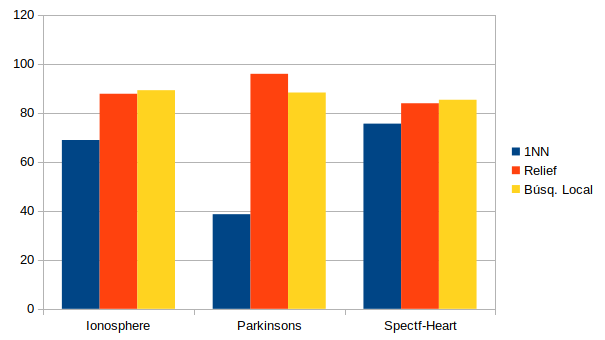
\includegraphics[width=0.55\textwidth]{images/tasa_clas.png}
		\caption{Tasa de clasificación.}
	\end{figure}
	
	Podemos observar que en general 1-NN ofrece peores tasas de clasificación, mientras que Relief y Búsq. Local alcanzan tasas similares. Esto tiene sentido pues en 1-NN se tiene que elegir el ejemplo o elemento más cercano usando todas las características mientras que con Relief y Búsq. Local, tras el ajuste de pesos, se tiene la posibilidad de no considerar ciertas características que probablemente no sean relevantes y solo estén introduciendo ``ruido'' en la clasificación (se descartan las de peso $< 0.2$).\\
	
	Vemos ahora las tasas de reducción:
	\begin{figure}[H]
		\centering
		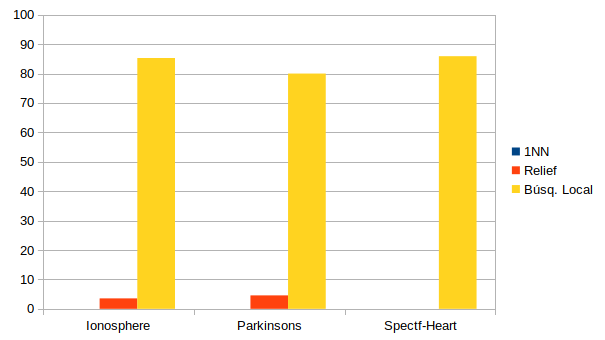
\includegraphics[width=0.55\textwidth]{images/tasa_red.png}
		\caption{Tasa de reducción.}
	\end{figure}
	
	Claramente las tasas de reducción con 1-NN son 0 por lo comentado. Se observa además una gran diferencia entre Búsq. Local y Relief, alcanzando mucha más reducción Búsq. Local. Esto también era de esperar pues en Búsq. Local, con $\alpha=5$ como nuestro caso, lo que se busca es un equilibrio entre tasa de clasificación y tasa de reducción (se va evaluando la función objetivo y es el criterio de elección) mientras que en Relief simplemente se van modificando los pesos en función de los amigos y enemigos más cercanos, la tasa de reducción no se tiene en cuenta en Relief.\\
	
	Por último el valor agregado:
	
	\begin{figure}[H]
		\centering
		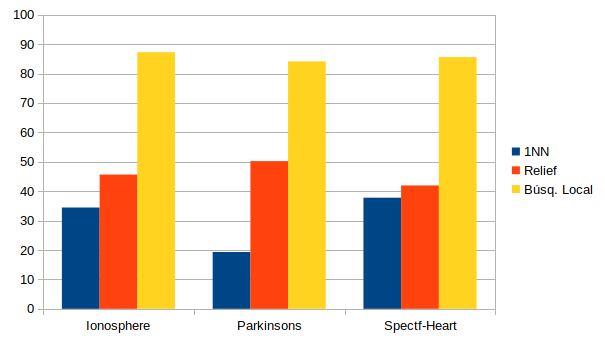
\includegraphics[width=0.55\textwidth]{images/agr.png}
		\caption{Valor de función objetivo o agregado.}
	\end{figure}
	
	Observamos una clara superioridad de Búsq. Local, seguido de Relief, y por último 1-NN. Era predecible pues 1-NN ha sido el que peores tasas ha mostrado, y aunque Búsq. Local y Relief tenían tasas de clasifiación similares, la tasa de reducción en Búsq. Local es mucho mayor que la de Relief.\\
	
	En cuanto a los tiempos:
	
		Como observamos en la tabla resumen, Relief es bastante rápido, tiene tiempos de ejecución similares a 1-NN y alcanza buenas tasas de clasificación, supone una gran mejora respecto a 1-NN. Búsq. Local sin embargo tiene tiempos de ejecución bastante superiores a ambos, aunque como hemos visto, los valores que se alcanzan en la función objetivo son muy superiores aunque sean de óptimos locales.
	

\end{document}
	

